\titledquestion{Topological Sorting}

Consider the unweighted directed graph $G$ below. 

\begin{figure}[H]
    \centering
    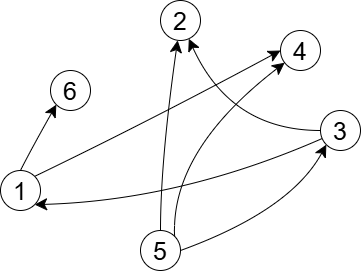
\includegraphics[width=0.5\linewidth]{fig/Topological_Sort.png}
    \label{fig:Topological_Sort}
\end{figure}

\begin{parts}

\part[5] 
How many topological sort results are there for the graph? State all possible results and show your calculated process.

\vspace{5cm}


\part[5] 
Construct an example of a single directed edge that, when added to $G$, would make it impossible to create a valid topological ordering of the graph. Then, determine the total number of such edges that could be added to $G$ and explain why each of these edges prevents a topological ordering.\\
(Ensure that this edge is not a self-loop and does not duplicate an existing edge in $G$.)

\vspace{5cm}

\end{parts}